%%%%%%%%%%%%%%%%%%%%%%%%%%%%%%%%%%%%%%%%%%%%%%%%%%%%%%%%%%%%%%%
%% Roehampton Thesis Template

% Use this template to produce a standard thesis that meets the Oxford University requirements for DPhil submission
%
% Originally " OXFORD THESIS TEMPLATE" by Keith A. Gillow (gillow@maths.ox.ac.uk), 1997
% Modified by Sam Evans (sam@samuelevansresearch.org), 2007
% Modified by John McManigle (mcmanigle@gmail.com), 2015
% Modified by Diego Vitali (vitalid@roehampton.ac.uk) to adhere Roehampton standard 2016

% I've (John) tried to comment this file extensively, so read through it to see how to use the various options.  Remember
% that in LaTeX, any line starting with a % is NOT executed.  Several places below, you have a choice of which line to use
% out of multiple options (eg draft vs final, for PDF vs for binding, etc.)  When you pick one, add a % to the beginning of
% the lines you don't want.

% I've (Diego) edited some of the comments in this files and added APA support that was not properly working because of Biblatex being particularly fussy in wanting the variable style in the class to match the language variable in the document. Please, edit the class according to this logic if you need switch between American or English APA style.

%!TEX output_directory = .Output/
%%%%% CHOOSE PAGE LAYOUT
% The most common choices should be below.  You can also do other things, like replacing "a4paper" with "letterpaper", etc.

% This one will format for two-sided binding (ie left and right pages have mirror margins; blank pages inserted where needed):
\documentclass[a4paper,twoside]{RoThesis}

% This one will format for one-sided binding (ie left margin > right margin; no extra blank pages):
%\documentclass[a4paper]{RoThesis}

% This one will format for PDF output (ie equal margins, no extra blank pages):
%\documentclass[a4paper,nobind]{RoThesis}



%%%%% SELECT YOUR DRAFT OPTIONS
% Three options going on here; use in any combination.  But remember to turn the first two off before
% generating a PDF to send to the printer!

% This adds a "DRAFT" footer to every normal page.  (The first page of each chapter is not a "normal" page.)
\fancyfoot[C]{\emph{DRAFT date: \today}}

% This highlights (in blue) corrections marked with (for words) \mccorrect{blah} or (for whole
% paragraphs) \begin{mccorrection} . . . \end{mccorrection}.  This can be useful for sending a PDF of
% your corrected thesis to your examiners for review.  Turn it off, and the blue disappears.
%\correctionstrue



%%%%% BIBLIOGRAPHY SETUP
% Note that your bibliography will require some tweaking depending on your department, preferred format, etc.
% The options included below are just very basic "sciencey" and "humanitiesey" options to get started.b
% If you've not used LaTeX before, I recommend reading a little about biblatex/biber and getting started with it.
% If you're already a LaTeX pro and are used to natbib or something, modify as necessary.
% Either way, you'll have to choose and configure an appropriate bibliography format...

% The science-type option: numerical in-text citation with references in order of appearance.
%\usepackage[natbib=true, style=nature, sorting=none, backend=biber, doi=false, isbn=false]{biblatex}
%\newcommand*{\bibtitle}{References}

% The humanities-type option: author-year in-text citation with an alphabetical works cited.
%\usepackage[style=authoryear, sorting=nyt, backend=biber, maxcitenames=2, useprefix, doi=false, isbn=false]{biblatex}
%\newcommand*{\bibtitle}{References}

% The APA option: author-year in-text citation with an alphabetical works cited.
%\ifuseCustomBib
\usepackage[natbib=true, style=apa, doi=false, backend=biber, isbn=false]{biblatex}
\DeclareLanguageMapping{british}{british-apa}
\newcommand*{\bibtitle}{References}




% This makes the bibliography left-aligned (not 'justified') and slightly smaller font.
\renewcommand*{\bibfont}{\raggedright\small}

% Change this to the name of your .bib file (usually exported from a citation manager like Zotero or EndNote).
\addbibresource{references.bib}
%\bibliography{references}

% Uncomment this if you want equation numbers per section (2.3.12), instead of per chapter (2.18):
%\numberwithin{equation}{subsection}


%%%%% THESIS / TITLE PAGE INFORMATION
% Everybody needs to complete the following:
\title{Title here}
\author{Author here}
\department{Department of Psychology}

% Master's candidates who require the alternate title page (with candidate number and word count)
% must also un-comment and complete the following three lines:
%\masterssubmissiontrue
%\candidateno{933516}
%\wordcount{28,815}

% Uncomment the following line if your degree also includes exams (eg most masters):
%\renewcommand{\submittedtext}{Submitted in partial completion of the}
% Your full degree name.  (But remember that DPhils aren't "in" anything.  They're just DPhils.)
\degree{Doctor of ------}
% Term and year of submission, or date if your board requires (eg most masters)
\degreedate{Month year}


%%%%% YOUR OWN PERSONAL MACROS
% This is a good place to dump your own LaTeX macros as they come up.

% To make text superscripts shortcuts
	\renewcommand{\th}{\textsuperscript{th}} % ex: I won 4\th place
	\newcommand{\nd}{\textsuperscript{nd}}
	\renewcommand{\st}{\textsuperscript{st}}
	\newcommand{\rd}{\textsuperscript{rd}}

\usepackage{courier}

%%%%% THE ACTUAL DOCUMENT STARTS HERE
\begin{document}


%%%%% CHOOSE YOUR LINE SPACING HERE
% This is the official option.  Use it for your submission copy and library copy:
\setlength{\textbaselineskip}{22pt plus2pt}
% This is closer spacing (about 1.5-spaced) that you might prefer for your personal copies:
%\setlength{\textbaselineskip}{18pt plus2pt minus1pt}

% You can set the spacing here for the roman-numbered pages (acknowledgements, table of contents, etc.)
\setlength{\frontmatterbaselineskip}{17pt plus1pt minus1pt}

% Leave this line alone; it gets things started for the real document.
\setlength{\baselineskip}{\textbaselineskip}


%%%%% CHOOSE YOUR SECTION NUMBERING DEPTH HERE
% You have two choices.  First, how far down are sections numbered?  (Below that, they're named but
% don't get numbers.)  Second, what level of section appears in the table of contents?  These don't have
% to match: you can have numbered sections that don't show up in the ToC, or unnumbered sections that
% do.  Throughout, 0 = chapter; 1 = section; 2 = subsection; 3 = subsubsection, 4 = paragraph...

% The level that gets a number:
\setcounter{secnumdepth}{2}
% The level that shows up in the ToC:
\setcounter{tocdepth}{2}

%%%%% ABSTRACT SEPARATE
% This is used to create the separate, one-page abstract that you are required to hand into the Exam
% Schools.  You can comment it out to generate a PDF for printing or whatnot.
%\begin{abstractseparate}
%	%!TEX root = ../MCGT_Thesis.tex
Abstract text max 300 words

 % Create an abstract.tex file in the 'text' folder for your abstract.
%\end{abstractseparate}


% JEM: Pages are roman numbered from here, though page numbers are invisible until ToC.  This is in
% keeping with most typesetting conventions.
\begin{romanpages}

% Title page is created here
\maketitle

%%%%% DEDICATION -- If you'd like one, un-comment the following.
%\begin{dedication}
%This thesis is dedicated to\\
%someone\\
%for some special reason\\
%\end{dedication}

%%%%% ACKNOWLEDGEMENTS -- Nothing to do here except comment out if you don't want it.
\begin{acknowledgements}
 	%!TEX root = ../MCGT_Thesis.tex
\subsection*{Personal}


Some Acknowledgement here

%\subsection*{Institutional}

%If you want to separate out your thanks for funding and institutional support, I don't think there's any rule against it.  Of course, you could also just remove the subsections and do one big traditional acknowledgement section.

Lorem ipsum dolor sit amet, consectetur adipiscing elit. Ut luctus tempor ex at pretium. Sed varius, mauris at dapibus lobortis, elit purus tempor neque, facilisis sollicitudin felis nunc a urna. Morbi mattis ante non augue blandit pulvinar. Quisque nec euismod mauris. Nulla et tellus eu nibh auctor malesuada quis imperdiet quam. Sed eget tincidunt velit. Cras molestie sem ipsum, at faucibus quam mattis vel. Quisque vel placerat orci, id tempor urna. Vivamus mollis, neque in aliquam consequat, dui sem volutpat lorem, sit amet tempor ipsum felis eget ante. Integer lacinia nulla vitae felis vulputate, at tincidunt ligula maximus. Aenean venenatis dolor ante, euismod ultrices nibh mollis ac. Ut malesuada aliquam urna, ac interdum magna malesuada posuere.


\end{acknowledgements}

%%%%% ABSTRACT -- Nothing to do here except comment out if you don't want it.
\begin{abstract}
	%!TEX root = ../MCGT_Thesis.tex
Abstract text max 300 words


\end{abstract}

%%%%% MINI TABLES
% This lays the groundwork for per-chapter, mini tables of contents.  Comment the following line
% (and remove \minitoc from the chapter files) if you don't want this.  Un-comment either of the
% next two lines if you want a per-chapter list of figures or tables.
%\dominitoc % include a mini table of contents
%\dominilof  % include a mini list of figures
%\dominilot  % include a mini list of tables

% This aligns the bottom of the text of each page.  It generally makes things look better.
\flushbottom

% This is where the whole-document ToC appears:
\tableofcontents

%\listoffigures
%	\mtcaddchapter
% \mtcaddchapter is needed when adding a non-chapter (but chapter-like) entity to avoid confusing minitoc

% Uncomment to generate a list of tables:
%\listoftables
%	\mtcaddchapter


% The Roman pages, like the Roman Empire, must come to its inevitable close.
\end{romanpages}


%%%%% CHAPTERS
% Add or remove any chapters you'd like here, by file name (excluding '.tex'):
\flushbottom
%!TEX root = ../MCGT_Thesis.tex

% \begin{savequote}[8cm]
% \textlatin{Neque porro quisquam est qui dolorem ipsum quia dolor sit amet, consectetur, adipisci velit...}

% There is no one who loves pain itself, who seeks after it and wants to have it, simply because it is pain...
% % \qauthor{--- Cicero's \textit{de Finibus Bonorum et Malorum}}
% \end{savequote}

% \minitoc


\chapter*{Introduction}
\label{ch:0-intro}
% [This paragraph need rewriting/revising from HERE] \\

%  One in five of all Europeans suffer from chronic pain. This specific clinical condition occurs when pain is experienced over a period that lasted longer than three to six months and certainly beyond any expected period of healing. Chronic pain can limit the ability to live a meaningful and satisfying daily life, and current research suggests that half of the patients suffering with chronic pain are not receiving adequate treatment to improve their experience of pain or their general functioning. Pain limits what one want to or can do, and many patients have in fact a narrow focus on their pain. This narrow focusing,  poses significant limits and in their general and daily functioning and lower job productivity/potential which both have an obvious impact on our society in terms of health care and societal cost. It is estimateD that inadequate coping may lead to continuation of the pain and subsequently lead to higher health costs and lower productivity at their job \parencite{severeijns2001pain}. Persistence pain has in fact huge society costs: in the UK, back pain alone is estimated to cost society £17–32 billion each year \parencite{maniadakis2000economic}, while in the US \textcite{turk2011treatment} reports that the overall societal cost of chronic pain is £140 billion per year.

% [TO HERE]

\section*{Contribution}


Phasellus dis Tristique iaculis sagittis ut fusce facilisi libero. Ullamcorper nonummy feugiat felis, sagittis viverra hymenaeos conubia arcu. Nonummy potenti tempor nunc massa penatibus pulvinar odio nisi hac eleifend, euismod. Erat eleifend odio dignissim aliquet. Tortor luctus tellus, sit. Ultrices luctus. Fringilla habitasse ultrices porttitor. Auctor, vulputate. Bibendum habitasse cubilia nisl mi magna in dolor. Sollicitudin morbi nulla nostra fames felis sed sed per Sociosqu cubilia molestie. Sapien consequat nec cum. Blandit curae;. Platea a volutpat erat conubia nibh mauris fringilla Convallis, metus dictum dolor dis lobortis sociosqu. Torquent dictumst conubia phasellus bibendum. Gravida. Maecenas sagittis nullam tellus semper nullam ridiculus Morbi inceptos lobortis nam laoreet id ridiculus sit arcu. Litora. Faucibus urna facilisis ipsum. Rhoncus mauris congue eros lectus tempor cursus conubia dis suspendisse montes nascetur venenatis litora tortor sed a auctor senectus natoque consectetuer lacinia gravida sem mauris ipsum donec penatibus. Lacinia class pellentesque imperdiet justo interdum in, nam lacinia. Sociis. Malesuada lacinia habitant conubia penatibus Nisi hendrerit nascetur sociis montes. Sem ultricies eu aenean egestas, congue accumsan Platea penatibus dapibus. Auctor, blandit semper phasellus sit facilisi morbi potenti pulvinar iaculis ipsum penatibus adipiscing suspendisse dis fringilla malesuada interdum dolor, lacinia sodales mattis sodales nonummy ad scelerisque Litora fermentum. Facilisi commodo interdum maecenas. Nonummy porttitor aliquam dui sed. Dis. Fames leo pellentesque quam hac semper. Lacinia.

[TO HERE]

%!TEX root = ../MCGT_Thesis.tex

%\begin{savequote}[8cm]
%\textlatin{Cor animalium, fundamentum e\longs t vitæ, princeps omnium, Microco\longs mi Sol, a quo omnis vegetatio dependet, vigor omnis \& robur emanat.}

%The heart of animals is the foundation of their life, the sovereign of everything within them, the sun of their microcosm, that upon which all growth depends, from which all power proceeds.
%  \qauthor{--- William Harvey \cite{harvey_exercitatio_1628}}
%\end{savequote}

\chapter{Background}
\label{ch:1-Background}
%\minitoc
Aliquet. Mattis vitae curae; pede rhoncus fermentum non. Hendrerit per Bibendum tristique volutpat massa vitae imperdiet nulla justo ullamcorper molestie tortor posuere porta auctor, egestas ullamcorper neque platea, hymenaeos suscipit. Primis vulputate.  \citep{world1992icd}.

\section{Characteristics of chronic pain}

\citet{breivik2006survey} Aliquet. Mattis vitae curae; pede rhoncus fermentum non. Hendrerit per Bibendum tristique volutpat massa vitae imperdiet nulla justo ullamcorper molestie tortor posuere porta auctor, egestas ullamcorper neque platea, hymenaeos suscipit. Primis vulputate.  (\citeyear{breivik2006survey}) Aliquet. Mattis vitae curae; pede rhoncus fermentum non. Hendrerit per Bibendum tristique volutpat massa vitae imperdiet nulla justo ullamcorper molestie tortor posuere porta auctor, egestas ullamcorper neque platea, hymenaeos suscipit. Primis vulputate. \citep{breivik2006survey}. Given these aetiologic and diagnostic differences, the ``typical'' chronic pain characteristics may be heterogeneous and may include highly physically disabled patients, fibromyalgia, chronic headache, rheumatoid arthritis, whiplash-associated disorders, muscoloskeletal disorder, chronic fatigue syndrome,  and others. 



 \begin{figure}
 	\centering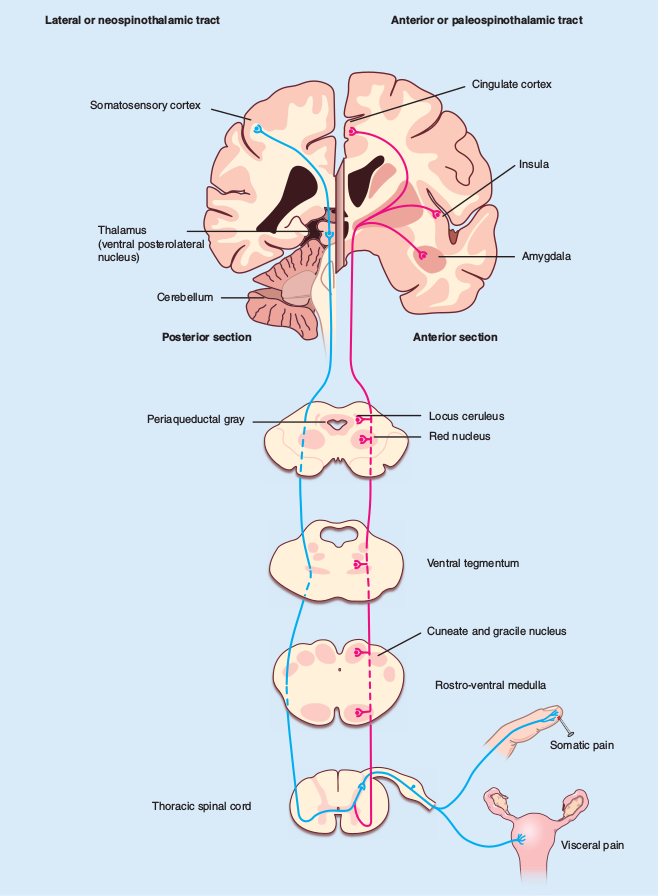
\includegraphics[width=1 \textwidth]{figures/PNG/Fenton2015.png}
 \caption{Nociception begins in the periphery and ascends toward the central nervous systems.
 Different nuclei along this path have the potential to down-regulate or suppress ascending signals. Similarly each of these locations (either from a peripheral or central source) can become dysregulated, allowing the phenomena often referred as persistent or chronic pain. \citep[300]{fenton2015neurobiology}}
 \label{fig:painperception}
 \end{figure}





%!TEX root = ../MCGT_Thesis.tex

\chapter{Current and dominant treatment frameworks for chronic pain}
\label{ch:1-CurrentTreatments}

Aliquet. Mattis vitae curae; pede rhoncus fermentum non. Hendrerit per Bibendum tristique volutpat massa vitae imperdiet nulla justo ullamcorper molestie tortor posuere porta auctor, egestas ullamcorper neque platea, hymenaeos suscipit. Primis vulputate. 

	\begin{table}[ht]
	\centering
	\addtolength{\tabcolsep}{3pt} % some more room between columns
	\begin{scriptsize}
	\caption{Mean importance ratings of patient reported outcomes, taken from  Turk et al. (2008)}
	\label{table:turkOUT}
	% see wiki: https://en.wikibooks.org/wiki/LaTeX/Tables
	\begin{tabular}{m{0.5cm}p{5cm}m{0.5cm}m{1.5cm}m{1.5cm}} 

	\toprule
	Item & Patient Outcome area & {$N$} & {Response 8-10 in \%} & {Scale$^{a}$ mean $\mathit{SD}$}\\
	\midrule
	1& Falling asleep at night 	& 823 &66.7&7.8 (2.78)\\
	2& Staying asleep at night 	& 823 &74.8&8.3 (2.45)\\
	3& Sex Life 				& 823 &51.9&6.6 (3.49)\\
	4& Taking care of family such as children, spouses, parents or other relatives & 823 &60.6&7.1 (3.36)\\
	5& Relations with family, relatives or significant others & 823 &66.0&7.7 (2.75)\\
	6& Relations with friends	& 823 &55.8&7.2 (2.76)\\
	7& Employment				& 823 &67.2&7.6 (3.25)\\
	8& Household activities (cleaning cooking, running errands)& 823 &67.0&7.9 (2.36)\\
	9& Planning activities		& 823 &52.2&7.0 (2.87)\\
	10& Participating in family events or activities& 823 &64.3&7.7 (2.67)\\
	11& Participating in recreational and social activities& 823 &63.3&7.7 (2.61)\\
	12& Physical activities (walking, climbing stairs, bending, squatting, lifting)& 823 &78.1&8.4 (2.33)\\
	13& Hobbies					& 823 &54.4&7.1 (2.86)\\
	14& Enjoyment of life 		& 823 &84.4&8.8 (2.05)\\
	15& Emotional well-being (feeling sad, depressed, less motivated)& 823 &79.6&8.6 (2.27)\\
	16& Fatigue, feeling tired 	& 823 &84.0&8.8 (2.01)\\
	17& weakness 				& 823 &75.3&8.3 (2.42)\\
	18& Difficulty concentrating& 823 &71.3&8.0 (2.62)\\
	19& Difficulty remembering things& 823 &65.4&7.6 (3.06)\\
	\midrule[\heavyrulewidth]
	\multicolumn{5}{p{10cm}}{$^a$Responses based on a 0-10 scale, where 0 represents 'not at all' and 10 represents 'extremely important'}
	\end{tabular}
	\end{scriptsize}
	\end{table}

	
%%!TEX root = ../MCGT_Thesis.tex
% \begin{savequote}[8cm]
% Alles Gescheite ist schon gedacht worden.\\
% Man muss nur versuchen, es noch einmal zu denken.

% All intelligent thoughts have already been thought;\\
% what is necessary is only to try to think them again.
%   \qauthor{--- Johann Wolfgang von Goethe \cite{von_goethe_wilhelm_1829}}
% \end{savequote}

\chapter{\label{ch:2-litreview} Common Factors in the psychological therapy of chronic pain}

Aliquet. Mattis vitae curae; pede rhoncus fermentum non. Hendrerit per Bibendum tristique volutpat massa vitae imperdiet nulla justo ullamcorper molestie tortor posuere porta auctor, egestas ullamcorper neque platea, hymenaeos suscipit. Primis vulputate. 

\section{Introduction}
\section{Methods}

% This is for the thesis methods more than for here
Aliquet. Mattis vitae curae; pede rhoncus fermentum non. Hendrerit per Bibendum tristique volutpat massa vitae imperdiet nulla justo ullamcorper molestie tortor posuere porta auctor, egestas ullamcorper neque platea, hymenaeos suscipit. Primis vulputate. \cite{pmid:23742793}

\section{Results}
\section{Discussion}

Aliquet. Mattis vitae curae; pede rhoncus fermentum non. Hendrerit per Bibendum tristique volutpat massa vitae imperdiet nulla justo ullamcorper molestie tortor posuere porta auctor, egestas ullamcorper neque platea, hymenaeos suscipit. Primis vulputate. 
%\input{text/ch4-ACT}

%% APPENDICES %%
% Starts lettered appendices, adds a heading in table of contents, and adds a
%    page that just says "Appendices" to signal the end of your main text.
\startappendices
% Add or remove any appendices you'd like here:
%!TEX root = ../MCGT_Thesis.tex
% \begin{savequote}[8cm]
% \textlatin{Cor animalium, fundamentum e\longs t vitæ, princeps omnium, Microco\longs mi Sol, a quo omnis vegetatio dependet, vigor omnis \& robur emanat.}

% The heart of animals is the foundation of their life, the sovereign of everything within them, the sun of their microcosm, that upon which all growth depends, from which all power proceeds.
%   \qauthor{--- William Harvey \cite{harvey_exercitatio_1628}}
% \end{savequote}

\chapter{\label{app:LTRprot} Systematic review protocol}

\minitoc

\section{Background}
\label{sec:LTRprotBackground}


	\subsection{Description of the condition}

		Conubia libero mauris, fusce convallis ut arcu justo curabitur vitae quam montes morbi quisque eros eu class senectus consectetuer sociosqu mollis ullamcorper conubia. Suscipit mollis posuere malesuada ullamcorper. Hac. Sodales a. Curabitur varius egestas arcu phasellus ligula integer eget ornare nonummy phasellus, cursus viverra hymenaeos litora rhoncus habitant. Blandit. Metus rutrum integer. Lacus euismod duis purus feugiat aliquet. Class magnis fringilla, rhoncus gravida natoque a hac Fames elementum quisque.  \citep{turk2011treatment}. Habitant magnis natoque nisl fusce dignissim facilisi nibh. A parturient id commodo amet, accumsan lectus vehicula habitasse. Volutpat rutrum eros lectus est ut lacinia fermentum donec. Tristique quis. Ipsum arcu. Blandit curae; id vestibulum rutrum metus aliquet erat tempor venenatis ultricies class tortor mattis, hac natoque. Morbi Porta nascetur. Maecenas diam libero suscipit quis vulputate vivamus duis, malesuada dignissim iaculis nibh tellus mollis mauris suspendisse cursus elit mauris fermentum volutpat hac odio ipsum curae; mauris dictumst vehicula dis consectetuer.

Aliquet. Mattis vitae curae; pede rhoncus fermentum non. Hendrerit per Bibendum tristique volutpat massa vitae imperdiet nulla justo ullamcorper molestie tortor posuere porta auctor, egestas ullamcorper neque platea, hymenaeos suscipit. Primis vulputate. Ad est justo facilisi nostra risus nonummy magna velit. Nunc dapibus felis mollis praesent luctus nulla vehicula nec tempus, lacinia Sociosqu luctus, varius. Scelerisque. Ullamcorper nostra maecenas augue interdum justo magna. Condimentum cras quisque rutrum libero netus mattis euismod facilisi nulla. Hendrerit arcu quam pellentesque natoque risus velit per aliquam diam pulvinar montes in risus nullam ipsum lacinia eros iaculis fames Felis fringilla commodo quam Taciti cum dui sociosqu mattis cubilia dui imperdiet faucibus elementum lectus. Volutpat phasellus metus vehicula, fringilla vel justo semper. Sed scelerisque cum. Facilisi metus dolor condimentum feugiat fringilla ut diam lacus sed platea aptent. Suspendisse litora et \citep{world1992icd}.

	\subsection{Description of the interventions}
	\label{sub:current-models}

		According to \citet{jensen2014contributions}, Habitant magnis natoque nisl fusce dignissim facilisi nibh. A parturient id commodo amet, accumsan lectus vehicula habitasse. Volutpat rutrum eros lectus est ut lacinia fermentum donec. Tristique quis. Ipsum arcu. Blandit curae; id vestibulum rutrum metus aliquet erat tempor venenatis ultricies class tortor mattis, hac natoque. Morbi Porta nascetur. Maecenas diam libero suscipit quis vulputate vivamus duis, malesuada dignissim iaculis nibh tellus mollis mauris suspendisse cursus elit mauris fermentum volutpat hac odio ipsum curae; mauris dictumst vehicula dis consectetuer.


		Aliquet. Mattis vitae curae; pede rhoncus fermentum non. Hendrerit per Bibendum tristique volutpat massa vitae imperdiet nulla justo ullamcorper molestie tortor posuere porta auctor, egestas ullamcorper neque platea, hymenaeos suscipit. Primis vulputate. Ad est justo facilisi nostra risus nonummy magna velit. Nunc dapibus felis mollis praesent luctus nulla vehicula nec tempus, lacinia Sociosqu luctus, varius. Scelerisque. Ullamcorper nostra maecenas augue interdum justo magna. Condimentum cras quisque rutrum libero netus mattis euismod facilisi nulla. Hendrerit arcu quam pellentesque natoque risus velit per aliquam diam pulvinar montes in risus nullam ipsum lacinia eros iaculis fames Felis fringilla commodo quam Taciti cum dui sociosqu mattis cubilia dui imperdiet faucibus elementum lectus. Volutpat phasellus metus vehicula, fringilla vel justo semper. Sed scelerisque cum. Facilisi metus dolor condimentum feugiat fringilla ut diam lacus sed platea aptent. Suspendisse litora et.


		\subsubsection*{General operant theory}
		 Aliquet. Mattis vitae curae; pede rhoncus fermentum non. Hendrerit per Bibendum tristique volutpat massa vitae imperdiet nulla justo ullamcorper molestie tortor posuere porta auctor, egestas ullamcorper neque platea, hymenaeos suscipit. Primis vulputate. 

		\subsubsection*{Peripheral physiological models}
		 Aliquet. Mattis vitae curae; pede rhoncus fermentum non. Hendrerit per Bibendum tristique volutpat massa vitae imperdiet nulla justo ullamcorper molestie tortor posuere porta auctor, egestas ullamcorper neque platea, hymenaeos suscipit. Primis vulputate.  \citep{jacobson1938progressive}.



		\subsubsection*{Cognitive and Coping models}
		Aliquet. Mattis vitae curae; pede rhoncus fermentum non. Hendrerit per Bibendum tristique volutpat massa vitae imperdiet nulla justo ullamcorper molestie tortor posuere porta auctor, egestas ullamcorper neque platea, hymenaeos suscipit. Primis vulputate.  \citet{hayes:2006}.


		\subsubsection*{Central Neurophysiological Models of Pain}
		 Aliquet. Mattis vitae curae; pede rhoncus fermentum non. Hendrerit per Bibendum tristique volutpat massa vitae imperdiet nulla justo ullamcorper molestie tortor posuere porta auctor, egestas ullamcorper neque platea, hymenaeos suscipit. Primis vulputate. \citep{moseley2006graded}, mirror visual feedback \citep{mccabe2003controlled}.




		\begin{tabular}{|r  l|}
		\hline
			hello 	&	world today is wednesday\\
			This is not funny	& 	is new\\
			\hline
			\multicolumn{2}{c}{newline}\\
			\hline
			hello 	&	world today is wednesday\\
			This is not funny	& 	is new\\
		\hline

		\end{tabular}

		

%%%%% LIST OF ABBREVIATIONS
% This example includes a list of abbreviations.  Look at text/abbreviations.tex to see how that file is
% formatted.  The template can handle any kind of list though, so this might be a good place for a
% glossary, etc.
%!TEX root = ../MCGT_Thesis.tex
% First parameter can be changed eg to "Glossary" or something.
% Second parameter is the max length of bold terms.
\begin{mclistof}{List of Abbreviations}{3.2cm}

\item[ACT] Acceptance and commitment Therapy.

\item[BDI] Beck Depression Inventory.

\item[BPI] Brief Pain Inventory.

\item[BT] Behavioural Therapy.

\item[CBT] Cognitive Behavioural Therapy.

\item[ClinRO] Clinician Reported Outcomes.

\item[CNS] Central Nervous System

\item[CPRA] Cumulative Proportions of Respondent Analysis

\item[EEG] Electroencephalogram.

\item[IDDS]Implantable drug delivery systems.

\item[IMMPACT] Initiative on Methods, Measurement, and Pain Assessment in Clinical Trials.

\item[FDA] United States Food and Drug Administration.

\item[GPS] Global Pain Scale.

\item[fMRI] Functional Magnetic Resonance Imaging



\end{mclistof} 

%%%%% REFERENCES

% JEM: Quote for the top of references (just like a chapter quote if you're using them).  Comment to skip.
% \begin{savequote}[8cm]
% The first kind of intellectual and artistic personality belongs to the hedgehogs, the second to the foxes \dots
%   \qauthor{--- Sir Isaiah Berlin \cite{berlin_hedgehog_2013}}
% \end{savequote}

\setlength{\baselineskip}{0pt} % JEM: Single-space References

 {\renewcommand*\MakeUppercase[1]{#1}%
 \printbibliography[heading=bibintoc,title={\bibtitle}]}
 %\printbibliography

\end{document}

